\documentclass[12pt, a4paper]{article}
\usepackage[utf8]{inputenc}
\usepackage[russian]{babel}
\usepackage[pdftex]{graphicx, color}
\usepackage{amsmath, amsfonts, amssymb, amsthm}
\usepackage[left=2cm,right=2cm,top=1.5cm,bottom=2cm]{geometry}
\usepackage{indentfirst}

\usepackage{setspace}
\onehalfspacing
\graphicspath{{pics/}}

\begin{document}

    \thispagestyle{empty}

    \begin{singlespace}
    \begin{titlepage}
        \begin{center}
            
\includegraphics[height = 3cm]{msu.png}

            {\scshape Московский государственный университет имени М.~В.~Ломоносова}\\
            Факультет вычислительной математики и кибернетики\\
            Кафедра математических методов прогнозирования\\
            \centerline{\hfill\hrulefill\hrulefill\hrulefill\hrulefill\hfill}

            \vfill

            {\LARGE Отчет ко второму практическому заданию по МОМО: \\ Продвинутые методы безусловной оптимизации}

            \vspace{1cm}

        \end{center}

        \vfill

        \begin{flushright}
            Студент 517 группы:\\
                \textit{Оспанов А.М.}

            \vspace{5mm}

        \end{flushright}

        \vfill

        \begin{center}
            Москва, 2016
        \end{center}
    \end{titlepage}
    \end{singlespace}

    \newpage

    \def \picwidth {17cm}
    \def \picheight {7.5cm}

    \section{Введение}
        В данной работе будут реализованы модули optim.py, lossfuncs.py, special.py с методами безусловной оптимизации и функциями потерь для логистической регрессии: метод сопряженных градиентов для решения системы линейных уравнений, нелинейный метод сопряженных градиентов, метод LBFGS и неточный метод Ньютона. Будут проведены исследования скорости сходимости метода сопряженных градиентов (CG) для различных чисел обусловленности матрицы системы. Также нелинейный метод сопряженных градиентов (NCG), метод LBFGS и неточный метод Ньютона (HFN) будут сравниваться между собой по невязке от вызова оракула и от времени работы циклов.

        Код написан на языке Python 3 с использованием библиотеки numpy.

    \section{Скорость сходимости метода сопряженных градиентов в зависимости от числа обусловленности $\kappa$ матрицы системы}
        Скорость сходимости метода будут исследоватся при $\kappa \in \{1.7, 17, 177\}$
        \begin{center}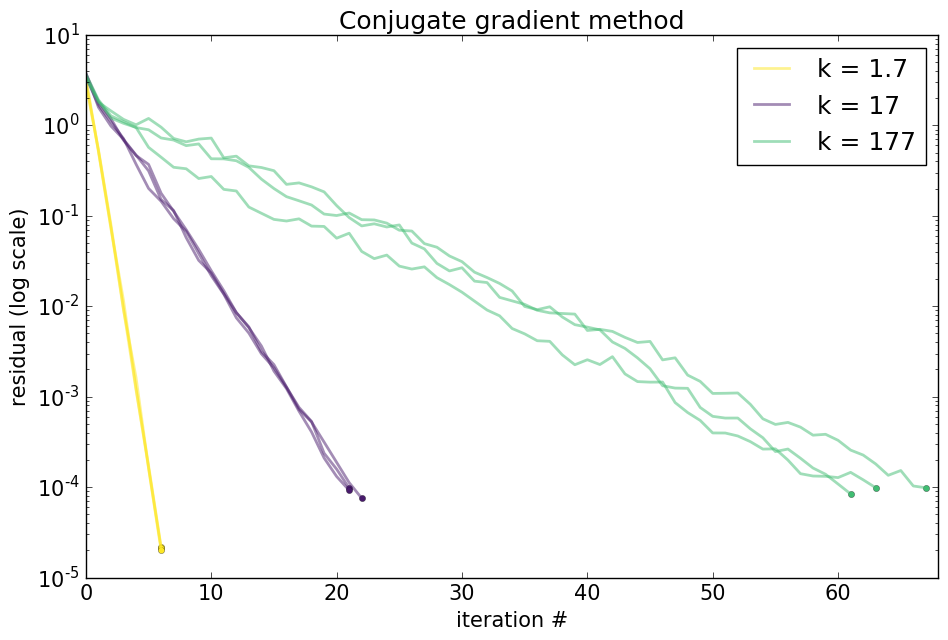
\includegraphics[width=\picwidth]{cg.png}\end{center}

        На графике видно, что чем больше $\kappa$, тем меньше скорость сходимости. Это объясняется особенностю метода CG: чем меньше различных собственных значений или чем меньше кластеров образуют собственные значения, тем быстрее метод сходится. Также очевидно, что чем меньше число обусловленности, тем меньше кластеров и/или меньше различных собственных значений. Т.о. скорость сходимости метода обратно пропорциональна числу обусловленности. Также стоит отметить, что скорость сходимости метода линейна.


    \section{Сравнение методов NCG, LBFGS и HFN}
        Сравниваться три реализованных метода будут на задачах обучения двухклассовой логистической регрессии на реальных данных. В качестве данных были выбраны:

        \begin{center}
        \begin{tabular}{ l | l }
            \bf{Data set} & \bf{(data size, feature size)}\\
            \hline
            svmguide1 & (3089, 4) \\
            a7a & (16100, 123) \\
            madelon & (2000, 500) \\
            gisette scale & (6000, 5000) \\
            leu & (38, 7129) \\
            rcv1 & (20242, 47236) \\
        \end{tabular}
        \end{center}

        Приведем все графики скоростей сходимости
        \def \picwidth {15cm}
        \begin{center}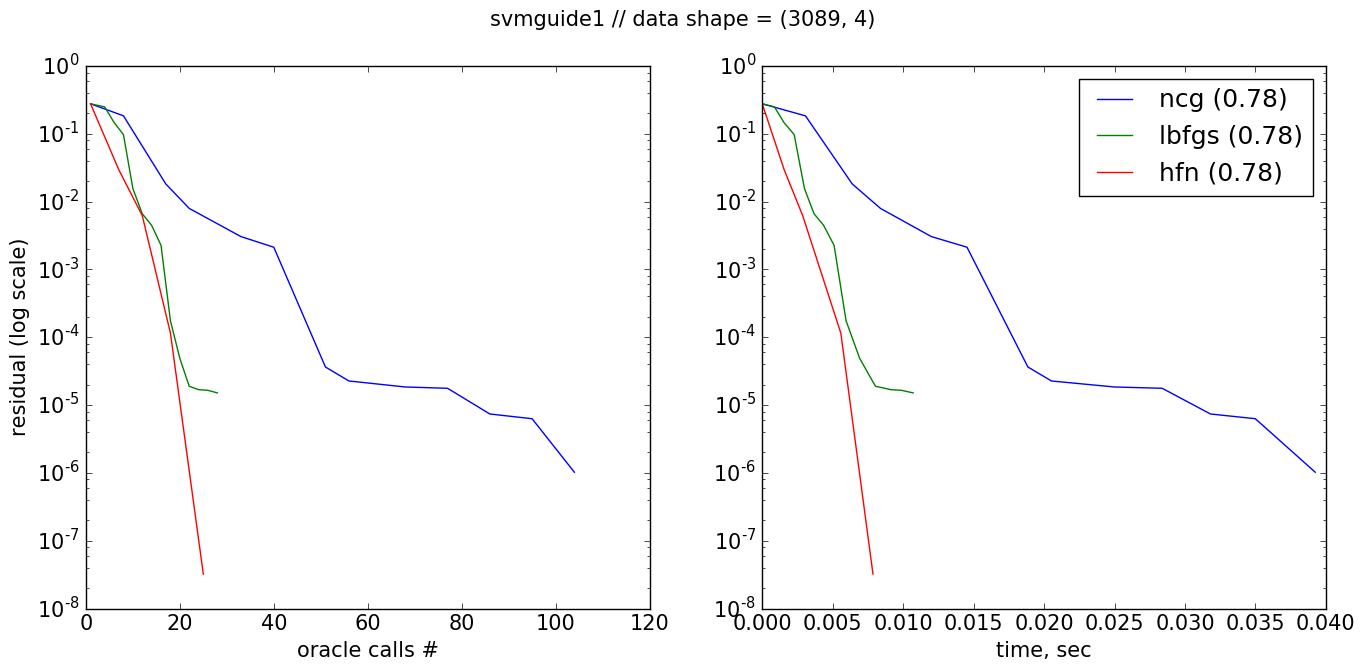
\includegraphics[width=\picwidth]{svmguide1.png}\end{center}
        \begin{center}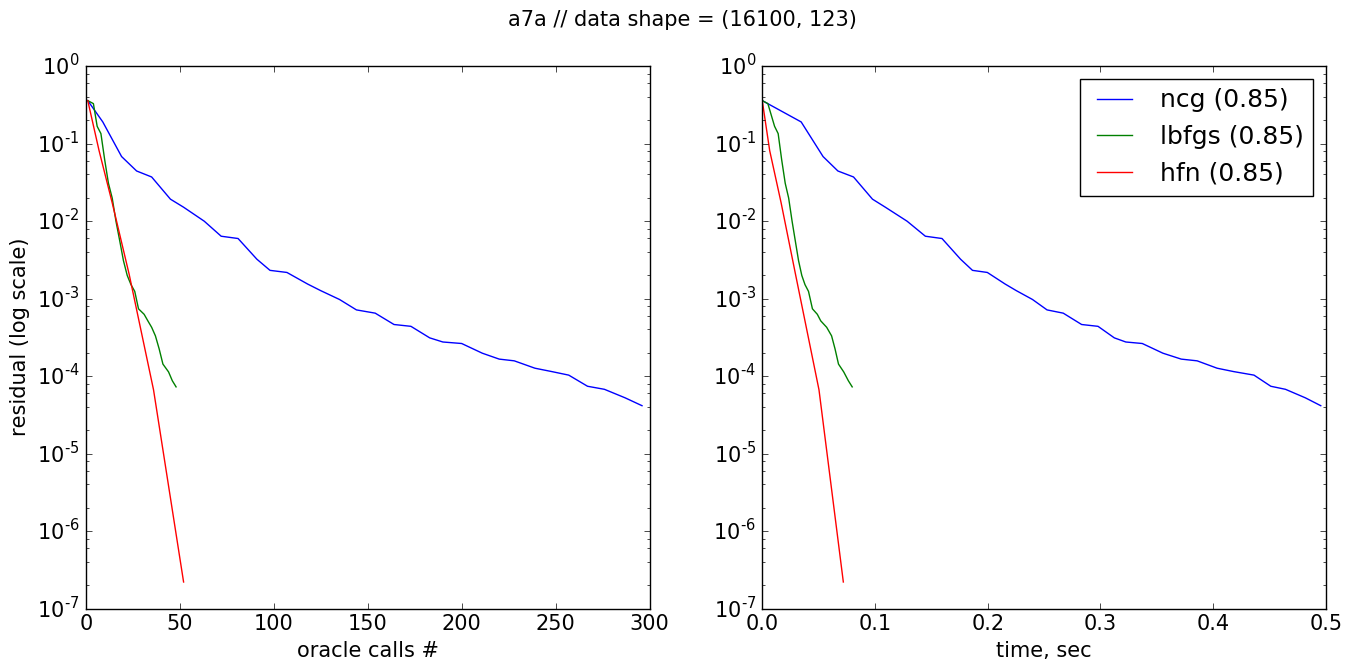
\includegraphics[width=\picwidth]{a7a.png}\end{center}
        \begin{center}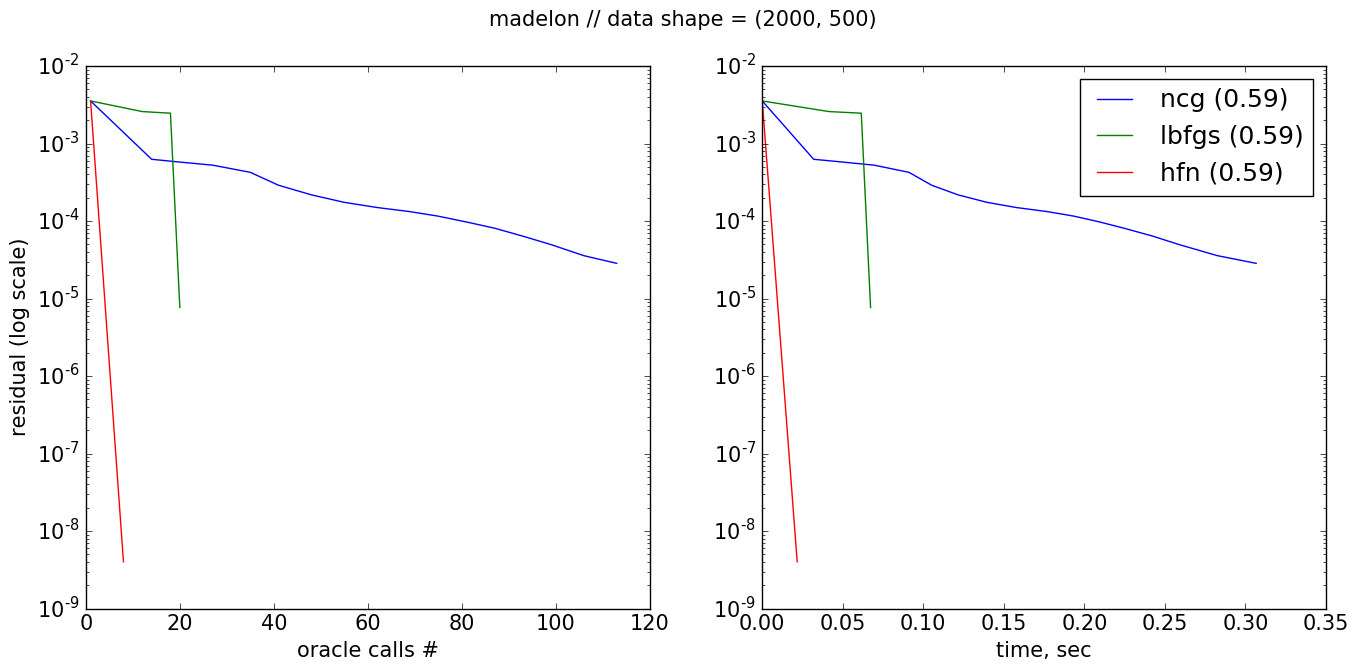
\includegraphics[width=\picwidth]{madelon.png}\end{center}
        \begin{center}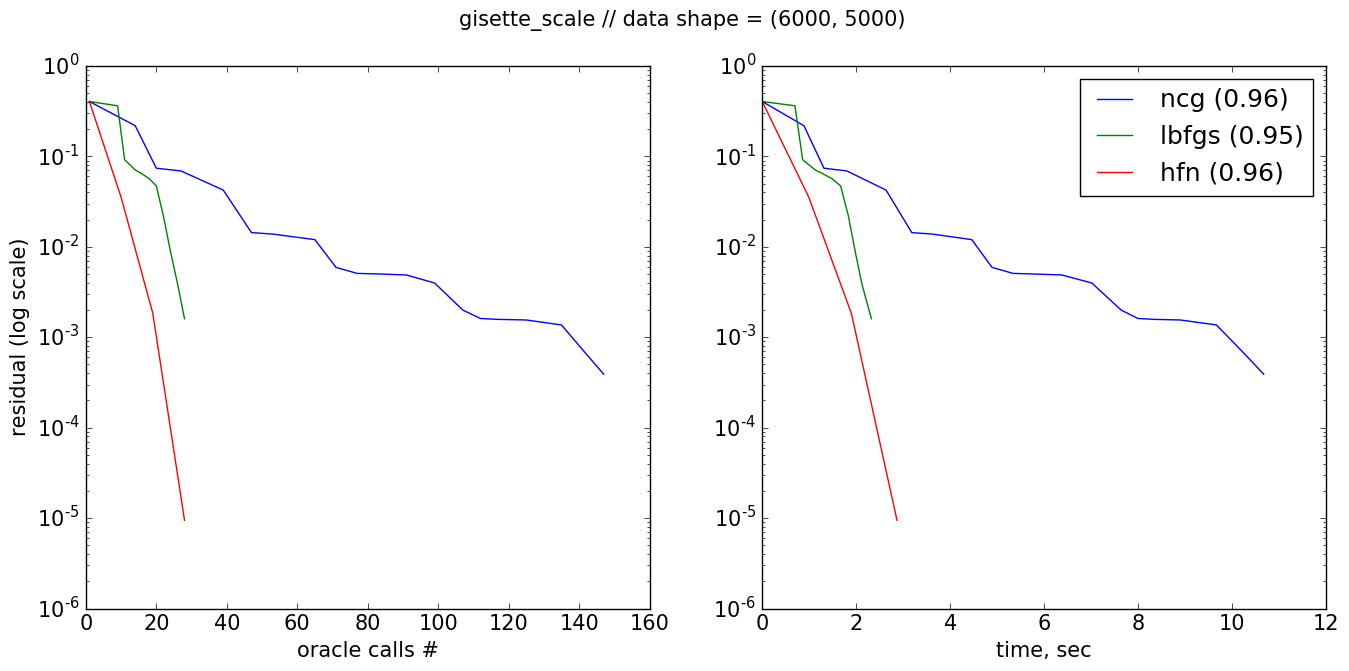
\includegraphics[width=\picwidth]{gisette_scale.png}\end{center}
        \begin{center}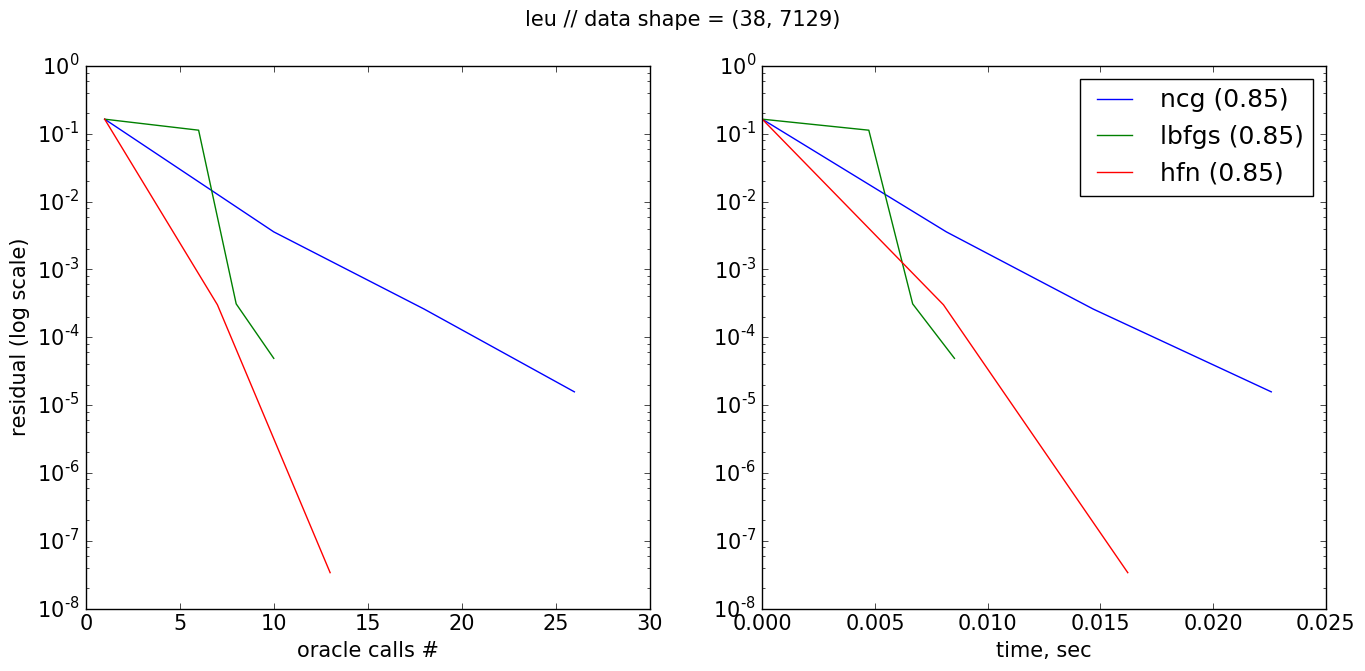
\includegraphics[width=\picwidth]{leu.png}\end{center}
        \begin{center}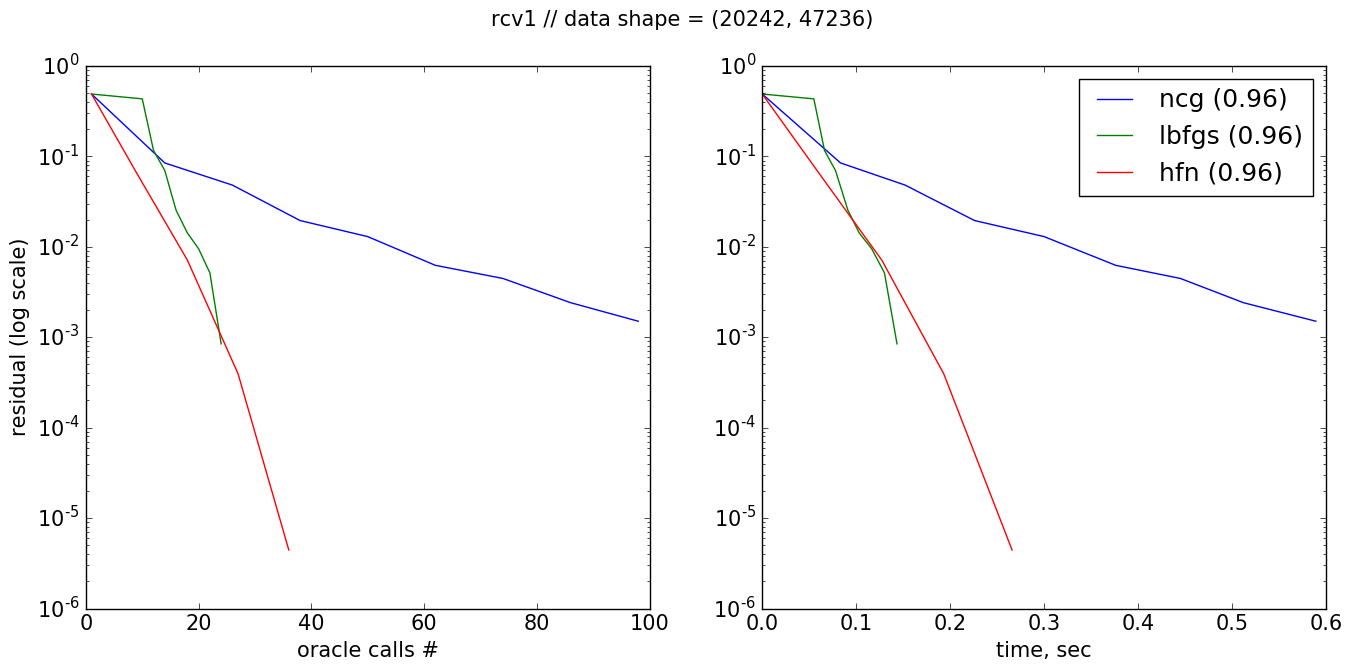
\includegraphics[width=\picwidth]{rcv1.png}\end{center}

        Из графиков видно, что метод NCG имеет сублинейную скорость сходимости, а HFN и LBFGS - суперлинейные скорости сходимости. В целом видно, что соотношения скоростей сходимости методов не меняются при увеличении количества признаков. Поэтому подробно рассмотрим только данные с маленьким и большим количество признаков.

        \def \picwidth {17cm}
        \begin{center}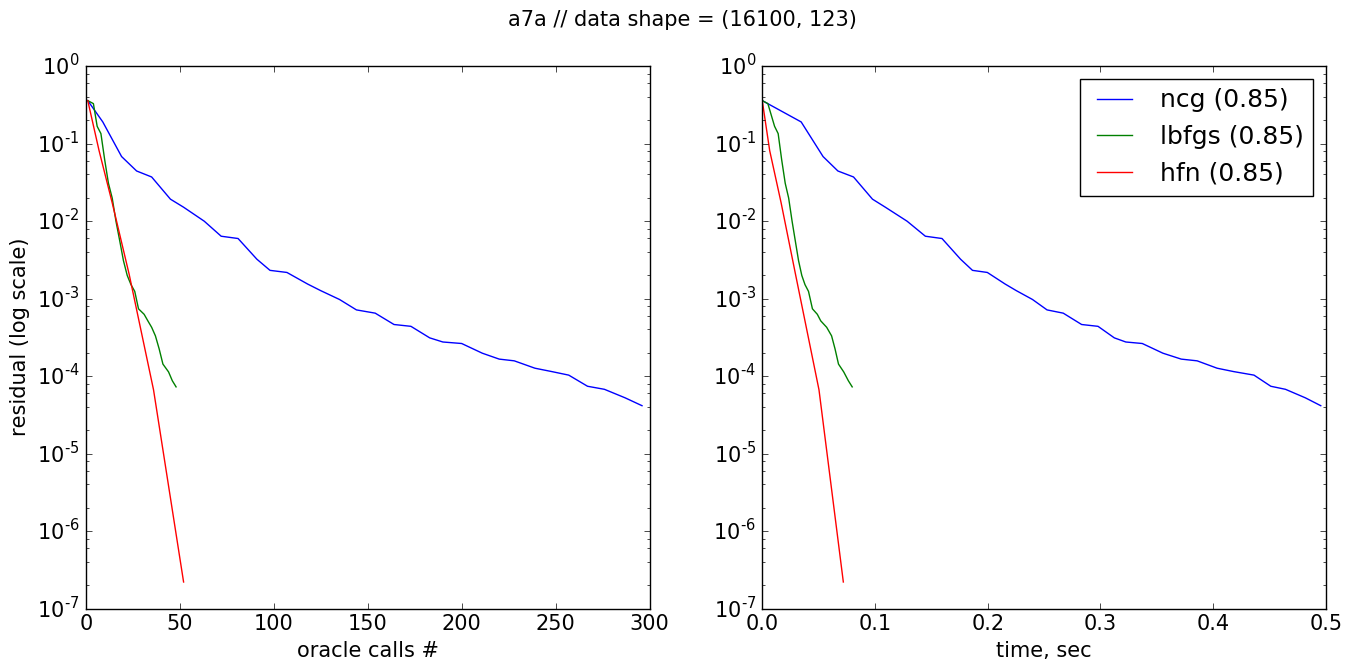
\includegraphics[width=\picwidth]{a7a.png}\end{center}

        Из графика понятно, что методы HFN и LBFGS на данных с маленьким количеством признаков работают одинаково и по количеству вызовов оракула и по времени работы. Но HFN дает большую точность. А метод NCG работает дольше в $\approx$5 раз, но при этом имеет невязку примерно как у LBFGS.

        \begin{center}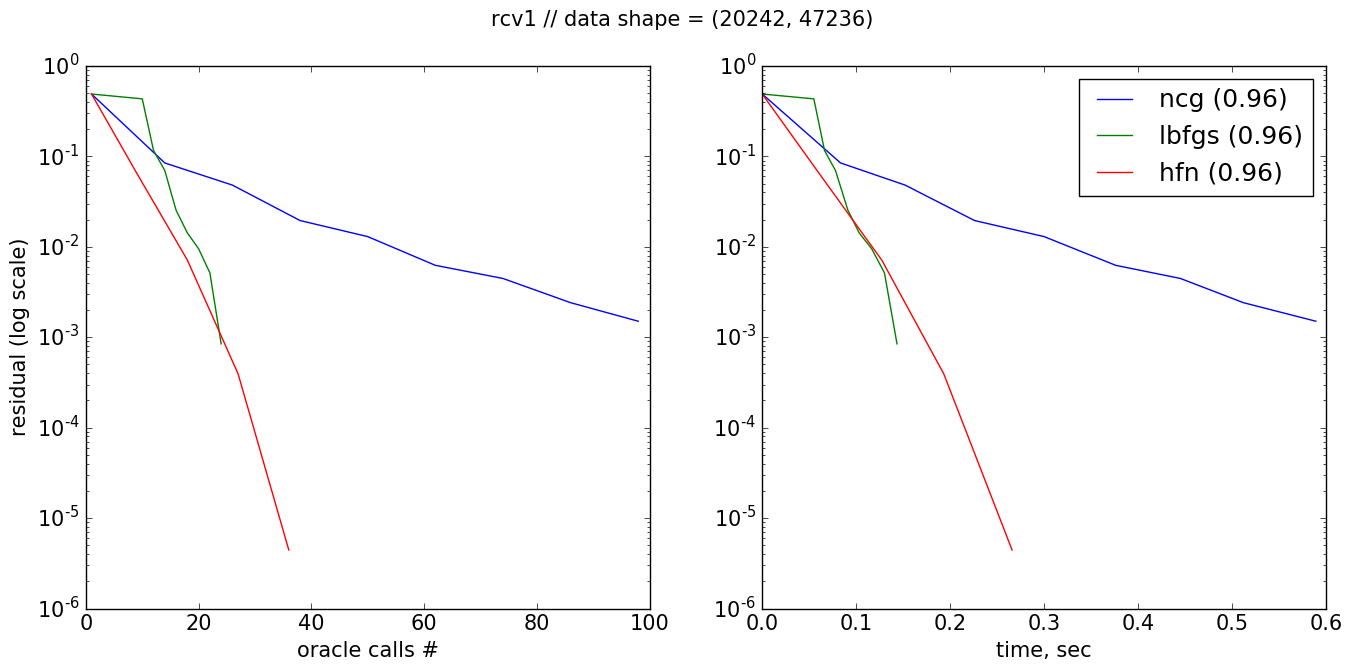
\includegraphics[width=\picwidth]{rcv1.png}\end{center}

        Как было замечено раньше, соотношения скоростей и точностей сохраняются. Соответственно, метод HFN является быстрым и самым точным. Метод LBFGS сходится быстрее всех, но менее точно. И метод NCG также выдает невязку примерно равную с LBFGS, но сходится дольше и также примерно в 5 раз.

        Из двух типов данных можно понять, что строгой зависимости между размерностью данных и скоростью работы методов не видно. Данные могут быть большой размерности, но сходиться быстрее, чем данные с меньшей размерностью. Скорость сходимости, скорее всего, зависит от природы данных.


    \section{Заключение}
        В работе сравнивались методы безусловной оптимизации. Были исследованы их скорости сходимости. В результате можно сказать:
        \begin{enumerate}
            \item Чем число обусловленности матрицы системы меньше, тем быстрее сходится метод CG;
            \item Метод HFN является достаточно быстрым и самым точным, в то время как NCG является самым не точным и самым медленным;
            \item Нет особой разницы в работе методов с данными большой и маленькой размерностей.
        \end{enumerate}

\end{document}
